\subsection*{Modelización 2}

Tenemos que construir un silo de forma cilíndrica para el almacenamiento de granos. La capacidad de almacenamiento del silo viene dada por la función $V(r, h)$, que depende de dos variables: radio de la base del silo ($r$) y su altura ($h$).

\begin{center}
    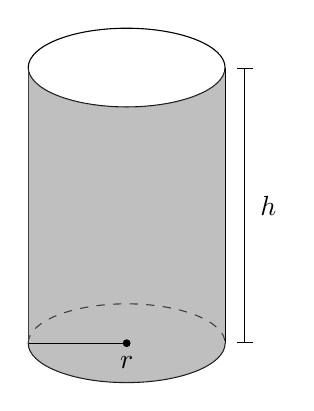
\begin{tikzpicture}
        \draw (0,0) ellipse (1.25 and 0.5);
        \draw (-1.25,0) -- (-1.25,-3.5);
        \draw (-1.25,-3.5) arc (180:360:1.25 and 0.5);
        \draw [dashed] (-1.25,-3.5) arc (180:360:1.25 and -0.5);
        \draw (1.25,-3.5) -- (1.25,0);
        \fill [gray,opacity=0.5] (-1.25,0) -- (-1.25,-3.5) arc (180:360:1.25 and 0.5) -- (1.25,0) arc (0:180:1.25 and -0.5);
        \draw (1.8,-1.75) node{$h$};
        \draw [|-|] (1.5,0) -- (1.5,-3.5);
        \draw (0,-3.75) node{$r$};
        \draw [line width=0.0mm] (-1.24,-3.5) -- (0,-3.5);
        \node at (0,-3.5) [circle,fill,inner sep=1pt]{};
    \end{tikzpicture}
\end{center}

Definimos la función de la capacidad de almacenamiento del silo como:

\begin{align*}
    V(r, h) & = \pi r^2h
\end{align*}

Por motivos estructurales incorporamos algunas restricciones. El radio no puede ser menor a 1 metro y la altura no puede superar los 24 metros. A su vez, por el material elegido, la altura no superar 3 veces el radio. La altura máxima para cada radio vendría dada por la expresión:

\begin{align*}
    3r & = h
\end{align*}

Si sustituimos en la expresión original:

\begin{align*}
    V & = \pi r^2 \cdot 3r \\
    V & = 3 \pi r^3
\end{align*}

Gráficamente:

\begin{center}
    \begin{tikzpicture}
        \begin{axis}[
                axis lines = left,
                xlabel = \(r\),
                ylabel = {\(V\)},
                clip = false,
                legend pos = outer north east,
                ymin = 0,
                xmin = 0,
            ]
            % volumen
            \addplot [
                domain=1:8,
                samples=200,
                color=orange,
            ]
            {3 * 3.14159265 * x * x * x};
            \addlegendentry{\(V = 3 \pi r^3\)}


        \end{axis}
    \end{tikzpicture}
\end{center}

Dadas las restricciones al radio y la altura, el dominio de la función sería $D = [1, 8]$.

Por su parte, la imagen sería $I = [9.43, 4825.49]$.
